\documentclass[14pt,a4paper]{article}
\renewcommand{\normalsize}{\fontsize{14pt}{16.8pt}\selectfont}
\usepackage[T2A]{fontenc}
\usepackage[utf8]{inputenc}
\usepackage[russian]{babel}
\usepackage{geometry}
\usepackage{setspace}
\usepackage{titlesec}
\usepackage{indentfirst}
\usepackage{amsmath}
\usepackage{graphicx}
\usepackage{float}
\usepackage{framed}
\usepackage{listings}
\usepackage{xcolor} 

\geometry{
  a4paper,
  left=30mm,
  right=15mm,
  top=20mm,
  bottom=20mm
}

% Настройка стилей
\titleformat{\section}[block]
  {\normalfont\fontsize{14}{16}\bfseries\centering}
  {\thesection.}{0.5em}{}
\titleformat{\subsection}[block]
  {\normalfont\fontsize{14}{16}\bfseries\filcenter}
  {\thesubsection.}{0.5em}{}
\titleformat{\subsubsection}[block]
  {\normalfont\fontsize{14}{16}\bfseries\filcenter}
  {\thesubsubsection.}{0.5em}{}

\lstset{
    basicstyle=\ttfamily\small,
    keywordstyle=\color{blue},
    commentstyle=\color{green},
    stringstyle=\color{red},
    frame=single,
    tabsize=4,
    showstringspaces=false,
    breaklines=true
}
  
\onehalfspacing

\setlength{\parindent}{1.25cm}

\begin{document}

\begin{titlepage}
\begin{center}

\onehalfspacing

\begin{center}
    \textbf{МИНИСТЕРСТВО НАУКИ И ВЫСШЕГО ОБРАЗОВАНИЯ РОССИЙСКОЙ ФЕДЕРАЦИИ} \\
    Федеральное государственное автономное образовательное учреждение высшего образования \\
    «Национальный исследовательский Нижегородский университет им. Н.И. Лобачевского» (ННГУ) \\
    Институт информационных технологий, математики и механики
\end{center}

\vspace{4cm}

\begin{center}
    \textbf{ОТЧЕТ ПО УЧЕБНОЙ ПРАКТИКЕ} \vspace{0.5cm}\\
    «Параллельные алгоритмы численного интегрирования» \vspace{0.5cm}\\
    по курсу «ПАРАЛЛЕЛЬНОЕ ПРОГРАММИРОВАНИЕ»
\end{center}

\vspace{4cm}

\begin{flushleft}
    \textbf{ВЫПОЛНИЛ} \\ 
    \begin{tabular}{@{}c@{}c@{}c@{}}
        Студент 3 курса группы  \hfill \underline{\hspace{3cm}} \hfill & \underline{\hspace{3cm}} & \underline{\hspace{3cm}} \\
        & \text{подпись} & \text{(Холин К.И.)} \\
    \end{tabular} \\
    \vspace{1cm}
    \textbf{ПРОВЕРИЛИ} \\
    \begin{tabular}{@{}c@{}c@{}c@{}}
        \underline{\hspace{5cm}} & \underline{\hspace{3cm}} & \underline{\hspace{3cm}} \\
        \text{(должность, уч. степень, звание)} & \text{подпись} & \text{(Фамилия И.О.)} \\
    \end{tabular} \\
    \begin{tabular}{@{}c@{}c@{}c@{}}
        \underline{\hspace{5cm}} & \underline{\hspace{3cm}} & \underline{\hspace{3cm}} \\
        \text{(должность, уч. степень, звание)} & \text{подпись} & \text{(Фамилия И.О.)} \\
    \end{tabular} \\
\end{flushleft}

\vspace{1cm}

\begin{center}
    Нижний Новгород 2025\newpage
\end{center}

\end{center}
\end{titlepage}

\tableofcontents
\newpage

\section{ВВЕДЕНИЕ}

При разработке программного обеспечения иногда возникают сложности времени исполнения. Для решения этой проблемы программисты используют подходы к созданию многопоточных программ, которые не уступают в производительности последовательной версии. В настоящем отчёте будут рассмотрены следующие технологии создания параллельных программ: OpenMP, TBB, std::thread, MPI + OpenMP.

\begin{flushleft}


\textit{Цель:} Создание параллельных программ и их анализ \\
\textit{Задачи:}
\begin{itemize}
\item Знакомство с задачей
\item Написание параллельных алгоритмов
\item Описание основных принципов работы технологий распараллеливания
\item Тестирование параллельных версий алгоритмов
\item Построение графиков эффективности работ параллельных программ
\item Сравнение полученных результатов и выводы
\end{itemize}

\textit{Объект исследования:} Вычислительные системы с общей памятью
\vspace{0.5cm}

\textit{Предмет исследования:} Технологии параллельного программирования
 (OpenMP, TBB, std::thread, MPI+OpenMP)
\vspace{0.5cm}

\textit{Методы исследования:} Анализ и обобщение
\end{flushleft}



\newpage

\section{ОСНОВНАЯ ЧАСТЬ}

\subsection{Постановка задачи}
\subsubsection{Одномерный случай}
Необходимо вычислить определённый интеграл на отрезке $[a, b]$. Этот отрезок разбивается на $n$ равных частей, где длина каждой части определяется как $h = \frac{b - a}{n}$. Здесь $b$ и $a$ - конец и начало отрезка, вместо которых подставляются пределы интегрирования, а $n$ - число шагов.

Обозначим через $f\left(x_{i-1} + \frac{h}{2}\right)$ значение функции в середине каждого частичного отрезка. Затем составим сумму произведений всех таких значений $f\left(x_{i-1} + \frac{h}{2}\right)$ на $h$ (шаг отрезка). Полученная сумма будет представлять собой приближённое значение определённого интеграла на отрезке $[a, b]$ по формуле средних прямоугольников:

\[
\int_{a}^{b} f(x) \, dx \approx h \sum_{i=1}^{n} f\left(x_{i-1} + \frac{h}{2}\right) = h \sum_{i=1}^{n} f\left(x_{i} - \frac{h}{2}\right).
\]

\begin{itemize}
\item Формула интегрирования: формула средних прямоугольников
\item Граничные условия: $a$ и $b$ - пределы интегрирования
\item Особенности решения: точность зависит от числа разбиений $n$
\end{itemize}

\subsubsection{Многомерный случай}
Задача аналогична задаче одномерного случая. $d$-мерная область интегрирования разбивается на равные части по каждому измерению. В центре каждой части вычисляется значение функции. Шаг по каждому измерению вычисляется как:

\[ h = \frac{b - a}{n} \]

где $b$ и $a$ - границы интегрирования по каждому измерению соответственно, $n$ - число шагов.

Общая формула для $d$-мерного интеграла методом средних прямоугольников:

\[ I \approx \sum_{i_1=1}^n \sum_{i_2=1}^n \dots \sum_{i_d=1}^n f(x_{i_1}, x_{i_2}, \dots, x_{i_d}) \cdot h^d \]

где координаты центров вычисляются как:

\[ x_{i_k} = a + \left(i_k - \frac{1}{2}\right) \cdot h, \quad k = 1, \dots, d \]

\subsection{Описание алгоритма}
Алгоритм вычисления многомерного интеграла методом средних прямоугольников заключается в следующем:

\begin{flushleft}
1. \textbf{Разбиение области интегрирования} \\
Область интегрирования разбивается на малые равные части по каждому измерению. Количество разбиений по каждому измерению задаётся параметром $n$, который определяет точность вычислений.

2. \textbf{Вычисление шага интегрирования} \\
Для каждого измерения определяется шаг интегрирования $h$ по формуле:
\[ h = \frac{b - a}{n} \]
где $a$ и $b$ - нижний и верхний пределы интегрирования по данному измерению соответственно.

3. \textbf{Определение точек вычисления} \\
В каждом подотрезке берётся средняя точка. Для многомерного случая вычисляются координаты центра каждого гиперпрямоугольника:
\[ x_k = a_k + \left(i_k + \frac{1}{2}\right) \cdot h_k, \quad k = 1,\ldots,d \]
где $d$ - размерность пространства.

4. \textbf{Вычисление суммы} \\
Значение подынтегральной функции вычисляется в центре каждого гиперпрямоугольника. Все полученные значения суммируются:
\[ I = \sum_{i_1=1}^n \cdots \sum_{i_d=1}^n f(x_1,\ldots,x_d) \]

5. \textbf{Учёт объёма} \\
Полученная сумма $I$ умножается на произведение шагов интегрирования по всем измерениям:
\[ \int\limits_{a_1}^{b_1} \cdots \int\limits_{a_d}^{b_d} f(x_1,\ldots,x_d) \,dx_1 \ldots dx_d \approx h_1 \cdot h_2 \cdot \ldots \cdot h_d \cdot I \]
\end{flushleft}

\subsection{Описание схемы параллельного алгоритма}
Во всех рассматриваемыыых технологиях в качестве участка распараллеливания выбирается
цикл внутри метода, отвечающего за интегрирование функции. 
\subsubsection{OpenMP}
Необходимо использовать директиву \texttt{\#pragma omp parallel for reduction(+:sum)}
 для автоматической редукции частичных интегральных сумм.
 Применение динамического распределения работы \texttt{dynamic}  между потоками допустимо,
 так как далеко не всегда вычисление интегральных сумм является лёгкой задачей,
 особенно для многомерного случая. Также возможны дополнительные накладные расходы на связь.

\subsubsection{TBB}
В качестве шаблонной функции распараллеливания следует использовать \texttt{tbb::parallel\_reduce} 
с одномерным итерационным пространством, поскольку нет вложенных циклов. Телом функции
\texttt{body} является цикл вычисления интегральной суммы.
Размер порции блока итераций \texttt{grain\_size}  установлен в 1000, чтобы минимизировать накладные расходы. 
Ответственность за распределение работы между потоками будет нести авто распределитель
(\texttt{auto\_partitioner}). Из операторов редукции выбрать сложение. 

\subsubsection{std::thread}
Достаточно выполнить распараллеливание цикла на первом уровне рекурсии.
Дальнейшее распараллеливание на уровнях ниже нецелесообразно, поскольку 
сильно усложнит реализацию(например, использование Threadpool) или приведёт 
к большим накладным расходам по созданию задач и новых потоков для них.

В текущем контексте реализация будет посложнее предыдущих, так как создание потоков
и распределение работы уже должен контролировать программист. Алгоритм 
распараллеливания следующий:

\begin{enumerate}
\item \textbf{Создание пула потоков} \\
Используется std::vector<std::thread>, где каждый поток обрабатывает свою часть интеграла.

\item \textbf{Ручное распределение работы} \\
Общее количество шагов (total\_steps) делится между потоками

\item \textbf{Запуск потоков} \\
Каждый поток получает свой диапазон [start, end):

\item \textbf{Сохранение результатов} \\
Частичные суммы сохраняются в массив thread\_sums[t].

\item \textbf{Синхронизация} \\
Основной поток ожидает завершения всех дочерних (th.join())
Затем суммируются результаты с помощью функции (std::accumulate)

\item \textbf{Учёт шага интегрирования} \\
Итоговая сумма умножается на величину шага h.
\end{enumerate}

\subsubsection{MPI + OpenMP}
Для процессов MPI нужно поделить отрезки интегрирования равномерно по каждой размерности между процессами. На следующем шаге использовать директиву \texttt{\#pragma omp parallel for} для распределения работы между потоками вектора шагов по каждой размерности внутри цикла. Применение директивы в текущем контексте уместно, поскольку позволит ускорить старт вычисления интегральных частичных сумм. После того, как вся работы между процессами и потоками будет распределена, начнутся вычисления. Подробный алгоритм приведён далее:

\begin{enumerate}
\item \textbf{Разделение области интегрирования (MPI)}
Каждый MPI-процесс получает свою часть отрезка.
Распределение выполняется только по первой размерности

\item \textbf{Синхронизация данных (MPI)}
Главный процесс (ранг 0) рассылает параметры.
Результаты собираются операцией $\mathtt{MPI\_Reduce}$ с $\mathtt{MPI\_SUM}$

\item \textbf{Масштаб (MPI)}
Для многомерных интегралов ($\mathtt{dim} > 1$) результат масштабируется:

\item \textbf{Параллельное вычисление шагов (OpenMP)}
Цикл расчета шагов интегрирования параллелизуется
директивой \texttt{\#pragma omp parallel for}

\item \textbf{Редукция (MPI)}
Локальные частичные суммы сводятся на главном процессе
Используется $\mathtt{MPI\_Reduce}$ с операцией суммирования
для сбора всех сумм.
\end{enumerate}

\subsection{Описание программной реализации}

\textbf{Настройка окружения:} 
\\
\textbf{a) через свойства системы}
\begin{enumerate}
\item Win + R. Открыть sysdm.cpl;
\item Дополнительно $\rightarrow$ Переменные среды;
\item В разделе "Переменные среды пользователя" создать переменную окружения;
\item Имя: OMP\_NUM\_THREADS. Значение: 4;
\item Нажать OK;
\end{enumerate}

\textbf{b) через PowerShell}

\begin{enumerate}
\item Открыть PowerShell;
\item Выполнить команду: \texttt{setx OMP\_NUM\_THREADS "4"};
\item Выполнить команду: \texttt{set OMP\_NUM\_THREADS=4};
\item Закрыть PowerShell;
\end{enumerate}


Детали реализации:
\subsubsection{OpenMP}

\textbf{Метод:}

\begin{framed}
\begin{lstlisting}[language=C++]
double Integrate(const Function& f, 
    const std::vector<double>& l_limits,
    const std::vector<double>& u_limits,
    const std::vector<double>& h,
    std::vector<double> f_values,
    int curr_index_dim, size_t dim, double n) 
{
    if (curr_index_dim == static_cast<int>(dim))
        return f(f_values);

    double sum = 0.0;
    
    #pragma omp parallel for reduction(+:sum) schedule(dynamic)
    for (int i = 0; i < static_cast<int>(n); ++i) {
        double coord = l_limits[curr_index_dim] + 
                      (i + 0.5) * h[curr_index_dim];
        f_values[curr_index_dim] = coord;
        
        sum += Integrate(f, l_limits, u_limits, h,
                       f_values, curr_index_dim+1, dim, n);
    }
    return sum * h[curr_index_dim];
}
\end{lstlisting}
\end{framed}

\textbf{Основные элементы и их назначение:}
\begin{itemize}
\item \texttt{\#pragma omp parallel for} - создание параллельной области
\item \texttt{reduction(+:sum)} - суммирование по потокам
\item \texttt{schedule(dynamic)} - динамическое распределение итераций цикла
\end{itemize}

\textbf{Требования к компиляции:}
\begin{enumerate}
\item Поддержка OpenMP (флаг \texttt{-fopenmp})
\item Уровень оптимизации \texttt{-O2}
\end{enumerate}

\subsubsection{TBB}
\textbf{Метод:}

\begin{framed}
\begin{lstlisting}[language=C++]
double Integrate(const Function& f, 
    const std::vector<double>& l_limits,
    const std::vector<double>& u_limits,
    const std::vector<double>& h,
    std::vector<double>& f_values,
    int curr_index_dim, size_t dim, double n) 
{
    if (curr_index_dim == static_cast<int>(dim))
        return f(f_values);

    const double step = h[curr_index_dim];
    const double start_pos = l_limits[curr_index_dim] + (0.5 * step);

    return tbb::parallel_reduce(
        tbb::blocked_range<int>(0, static_cast<int>(n), 0.0,
        [&](const tbb::blocked_range<int>& r, double local_sum) {
            std::vector<double> local_f_values = f_values;
            for (int i = r.begin(); i < r.end(); ++i) {
                local_f_values[curr_index_dim] = 
                    start_pos + static_cast<double>(i) * step;
                local_sum += Integrate(f, l_limits, u_limits, h,
                    local_f_values, curr_index_dim + 1, dim, n);
            }
            return local_sum;
        },
        std::plus<>(), tbb::auto_partitioner()) * step;
}
\end{lstlisting}
\end{framed}


\textbf{Основные элементы и их назначение:}
\begin{itemize}
\item \texttt{tbb::parallel\_reduce} - шаблонная функция редукции из TBB
\item \texttt{tbb::blocked\_range} - одномерное итерационое пространство
\item \texttt{auto\_partitioner} - автоматическое распределение вычислений
\item \texttt{Лямбда-функция с захватом контекста по ссылке}
\end{itemize}

\textbf{Требования к компиляции:}
\begin{enumerate}
\item подключить библиотеку TBB
\item флаги: \texttt{-ltbb}
\end{enumerate}

\subsubsection{std::thread}
\textbf{Метод:}

\begin{framed}
\begin{lstlisting}[language=C++]
double Integrate(const Function& f,
    const std::vector<double>& l_limits,
    const std::vector<double>& u_limits,
    const std::vector<double>& h,
    std::vector<double> f_values,
    int curr_index_dim, size_t dim, double n)
{
    if (curr_index_dim == static_cast<int>(dim))
        return f(f_values);

    const int total_steps = static_cast<int>(n);
    double sum = 0.0;

    if (curr_index_dim == 0) {
        const int num_threads = ppc::util::GetPPCNumThreads();
        std::vector<std::thread> threads(num_threads);
        std::vector<double> thread_sums(num_threads, 0.0);

        const int base_steps = total_steps / num_threads;
        const int remainder = total_steps % num_threads;

        for (int t = 0; t < num_threads; ++t) {
            const int start = (t * base_steps) + 
                (t < remainder ? t : remainder);
            const int end = start + base_steps + 
                (t < remainder ? 1 : 0);

            threads[t] = std::thread([&, start, end, t]() {
                std::vector<double> local_f_values = f_values;
                double local_sum = 0.0;
                for (int i = start; i < end; ++i) {
                    local_f_values[0] = l_limits[0] + 
                        (i + 0.5) * h[0];
                    local_sum += Integrate(f, l_limits, u_limits, h,
                        local_f_values, 1, dim, n);
                }
                thread_sums[t] = local_sum;
            });
        }

        for (auto& th : threads) {
            if (th.joinable()) th.join();
        }
        sum = std::accumulate(thread_sums.begin(), 
            thread_sums.end(), 0.0) * h[0];
    } else {
        for (int i = 0; i < total_steps; ++i) {
            f_values[curr_index_dim] = l_limits[curr_index_dim] + 
                (i + 0.5) * h[curr_index_dim];
            sum += Integrate(f, l_limits, u_limits, h,
                f_values, curr_index_dim + 1, dim, n);
        }
        sum *= h[curr_index_dim];
    }
    return sum;
}
\end{lstlisting}
\end{framed}

\textbf{Основные элементы и их назначение:}
\begin{enumerate}
\item Создание пула потоков \texttt{std::vector<std::thread>}
\item \texttt{base\_steps} - число шагов для каждого потока
\item \texttt{remainder} - остаток, если число потоков нечётно
\item \texttt{start} - начало частичного отрезка интегрирования
\item \texttt{end} - конец частичного отрезка интегрирования
\item  \texttt{Лямбда-функция с захватом контекста по ссылке}
\item \texttt{th.join()} - функция блокировки основного потока
\item Использование \texttt{std::accumulate} для суммирования результатов
\end{enumerate}

\textbf{Требования к компиляции:}
\begin{enumerate}
\item Поддержка C++11 или новее
\item Флаг \texttt{-pthread}
\item Оптимизация \texttt{-O2}
\end{enumerate}

\subsubsection{MPI + OpenMP}
\textbf{Методы:}

\begin{framed}
\begin{lstlisting}[language=C++]
bool TestTaskALL::RunImpl() {
    int size, rank;
    MPI_Comm_size(MPI_COMM_WORLD, &size);
    MPI_Comm_rank(MPI_COMM_WORLD, &rank);

    if (rank == 0) {
        dim_ = *reinterpret_cast<int*>(task_data->inputs[0]);
        f_values_.assign(reinterpret_cast<double*>
(task_data->inputs[1]),
                       reinterpret_cast<double*>(task_data->inputs[1]) + sz_values_);
        lower_limits_.assign(reinterpret_cast<double*>
(task_data->inputs[2]),
                          reinterpret_cast<double*>
(task_data->inputs[2]) + sz_lower_limits_);
        upper_limits_.assign(reinterpret_cast<double*>
(task_data->inputs[3]),
                          reinterpret_cast<double*>
(task_data->inputs[3]) + sz_upper_limits_);
        start_n_ = *reinterpret_cast<double*>(task_data->inputs[4]);
    }

    MPI_Bcast(&sz_values_, 1, MPI_INT, 0, MPI_COMM_WORLD);
    MPI_Bcast(&sz_lower_limits_, 1, MPI_INT, 0, MPI_COMM_WORLD);
    MPI_Bcast(&sz_upper_limits_, 1, MPI_INT, 0, MPI_COMM_WORLD);
    MPI_Bcast(&dim_, 1, MPI_INT, 0, MPI_COMM_WORLD);
    MPI_Bcast(&start_n_, 1, MPI_DOUBLE, 0, MPI_COMM_WORLD);

    if (rank > 0) {
        f_values_.resize(sz_values_);
        lower_limits_.resize(sz_lower_limits_);
        upper_limits_.resize(sz_upper_limits_);
    }

    MPI_Bcast(lower_limits_.data(), sz_lower_limits_,
    MPI_DOUBLE, 0, MPI_COMM_WORLD);
    MPI_Bcast(upper_limits_.data(), sz_upper_limits_, 
    MPI_DOUBLE, 0, MPI_COMM_WORLD);
    MPI_Bcast(f_values_.data(), sz_values_, 
    MPI_DOUBLE, 0, MPI_COMM_WORLD);

    RunMultistepSchemeMethodRectangle(f_, f_values_, lower_limits_,
                                    upper_limits_, dim_, start_n_);
    return true;
}
\end{lstlisting}
\end{framed}

\begin{framed}
\begin{lstlisting}[language=C++]
double TestTaskALL::RunMultistepSchemeMethodRectangle(
    const Function& f, std::vector<double>& f_values,
    const std::vector<double>& l_limits,
    const std::vector<double>& u_limits,
    int dim, double n) {
    
    int rank, size;
    MPI_Comm_rank(MPI_COMM_WORLD, &rank);
    MPI_Comm_size(MPI_COMM_WORLD, &size);

    local_l_limits_.resize(dim);
    local_u_limits_.resize(dim);

    for (int i = 0; i < dim; ++i) {
        double range = u_limits[i] - l_limits[i];
        local_l_limits_[i] = l_limits[i] + (rank * range / size);
        local_u_limits_[i] = l_limits[i] + ((rank + 1) * range / size);
    }

    double local_result = IntegrateWithRectangleMethod(f, f_values, 
                            local_l_limits_, local_u_limits_, dim, n);

    if (dim > 1) {
        local_result *= std::pow(size, dim - 1);
    }

    MPI_Reduce(&local_result, &I_2n_, 1, MPI_DOUBLE, 
              MPI_SUM, 0, MPI_COMM_WORLD);
    return I_2n_;
}
\end{lstlisting}
\end{framed}


\begin{framed}
\begin{lstlisting}[language=C++]
double TestTaskALL::IntegrateWithRectangleMethod(
    const Function& f, std::vector<double>& f_values,
    const std::vector<double>& l_limits,
    const std::vector<double>& u_limits,
    int dim, double n) {
    
    std::vector<double> h(dim);
    #pragma omp parallel for
    for (int i = 0; i < dim; ++i) {
        h[i] = (u_limits[i] - l_limits[i]) / n;
    }
    return Integrate(f, l_limits, u_limits, h, f_values, 0, dim, n);
}

double TestTaskALL::Integrate(
    const Function& f, const std::vector<double>& l_limits,
    const std::vector<double>& u_limits, const std::vector<double>& h,
    std::vector<double>& f_values, int curr_index_dim, 
    int dim, double n) {
    
    if (curr_index_dim == dim) {
        return f(f_values);
    }

    double sum = 0.0;
    const double l_limit = l_limits[curr_index_dim];
    const double step = h[curr_index_dim];

    for (int i = 0; i < static_cast<int>(n); ++i) {
        f_values[curr_index_dim] = l_limit + 
            (static_cast<double>(i) + 0.5) * step;
        sum += Integrate(f, l_limits, u_limits, h, f_values, 
                        curr_index_dim + 1, dim, n);
    }
    return sum * h[curr_index_dim];
}
\end{lstlisting}
\end{framed}

\textbf{Основные элементы и их назначение:}
\begin{enumerate}
\item \texttt{RunImpl - инициализация хранилищ данных и их рассылка}:
  \begin{itemize}
  \item \texttt{MPI\_Bcast} - широковещательная рассылка данных \\
   Вектора для рассылки и их размеры :
  \begin{enumerate}
  \item \texttt{f\_values} - значения функции
  \item \texttt{lower\_limits\_} - нижние пределы интегрирования
  \item \texttt{upper\_limits\_} - верхние пределы интегрирования
  \item \texttt{sz\_values} - кол-во переменных функции
  \item \texttt{dim\_} - размерность
  \item \texttt{start\_n\_} - общее кол-во шагов интегрирования
  \end{enumerate}
  \end{itemize}

\item \texttt{RunMultistepSchemeMethodRectangle} - распределение данных:
  \begin{itemize}
  \item \texttt{local\_u\_limits\_} - локальные верхние пределы интегрирования для каждого процесса
  \item \texttt{local\_l\_limits\_} - локальные нижние пределы интегрирования для каждого процесса
  \item \texttt{MPI\_Reduce} - сбор всех \texttt{local\_result} в переменной \texttt{I\_2n\_}
  \begin{enumerate}
   \item \texttt{local\_result} - локальная частичная интегральная сумма
   \item \texttt{I\_2n} - финальный результат интегрирования
  \end{enumerate}
  \end{itemize}

\item \texttt{IntegrateWithRectangleMethod} - определение шагов интегрирования:
  \begin{itemize}
  \item \texttt{\#pragma omp parallel for} - параллелизация цикла по вычислению шагов по каждому измерению
  \begin{enumerate}
  \item \texttt{h} - вектор шагов интегрирования
  \end{enumerate}
  \end{itemize}

\item \texttt{Integrate} - интегрирование:
  \begin{itemize}
  \item \texttt{curr\_index\_dim == dim} - база рекурсии
  \item \texttt{f()} - подынтегральная функция
  \item \texttt{sum} - частичная сумма по текущему измерению
  \item \texttt{l\_limit} - нижний предел интегрирования по измерению
  \item \texttt{step} - шаг интегрирования по измерению
  \end{itemize}
\end{enumerate}

\textbf{Требования к компиляции:}
\begin{itemize}
\item Полный набор флагов: \texttt{mpic++ -fopenmp -O2 -std=c++17 -pthread -ltbb}
\item Библиотеки: OpenMPI, TBB
\item Точное соответствие стандарту C++17
\end{itemize}

\subsection{Результаты экспериментов}
Были исследованы три сценария работы алгоритма с различными объёмами данных:

\begin{figure}[H]
\centering
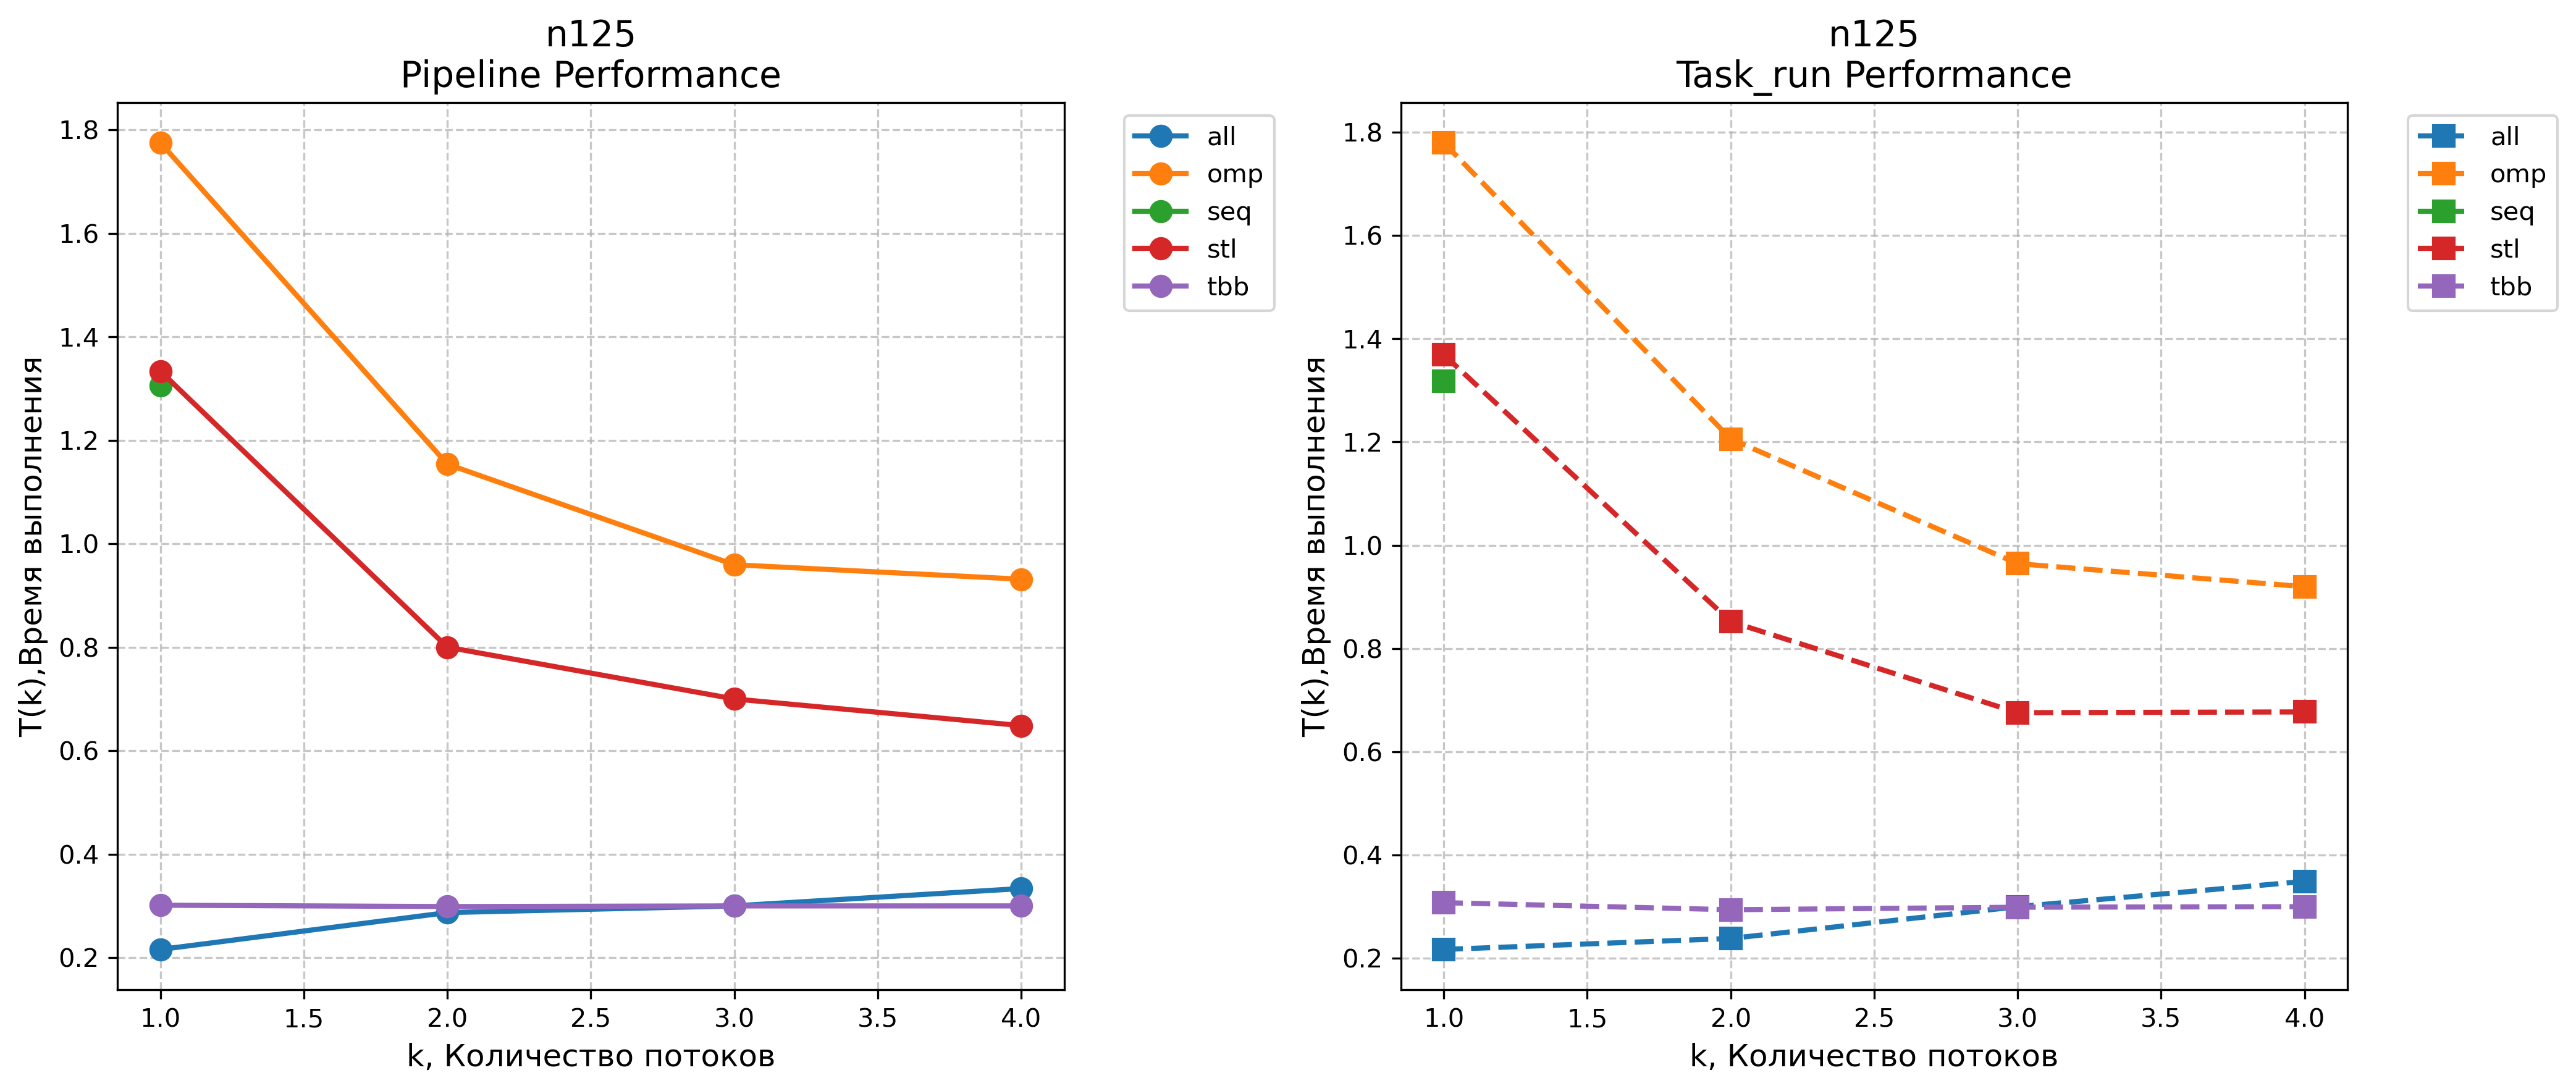
\includegraphics[width=0.8\textwidth]{C:/ppc-2025-threads-reports/tasks/kholin_k_multidim_integrals_rect/ppc_tests/graphics/performance_n125.png}
\caption{Графики производительности для малого объёма данных (n=125)}
\label{fig:small}
\end{figure}

\begin{figure}[H]
\centering
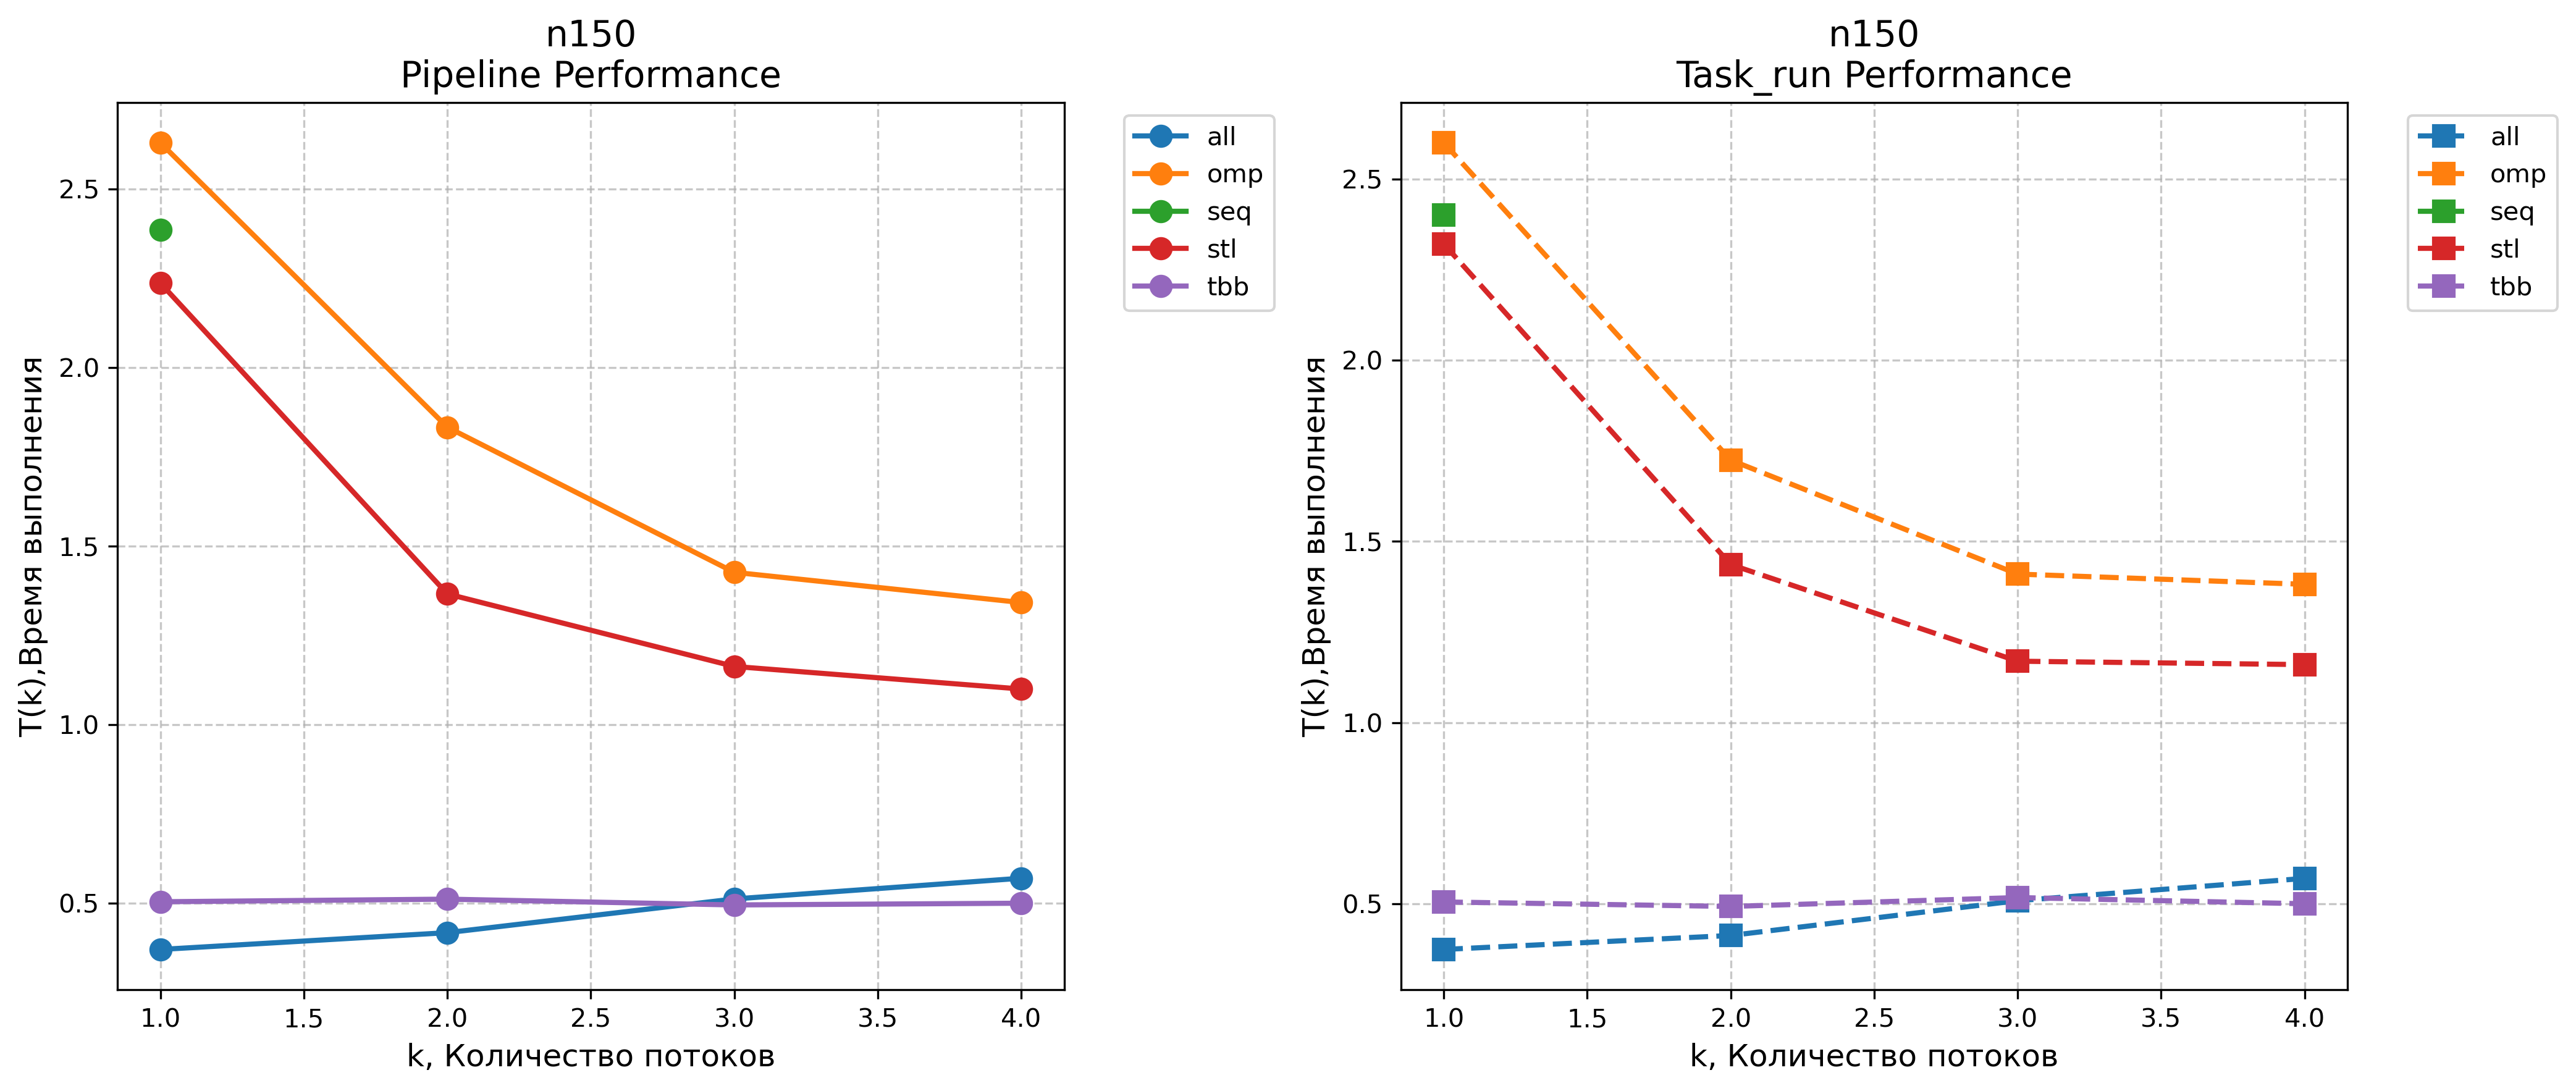
\includegraphics[width=0.8\textwidth]{C:/ppc-2025-threads-reports/tasks/kholin_k_multidim_integrals_rect/ppc_tests/graphics/performance_n150.png}
\caption{Графики производительности для среднего объёма данных (n=150)}
\label{fig:medium}
\end{figure}

\begin{figure}[H]
\centering
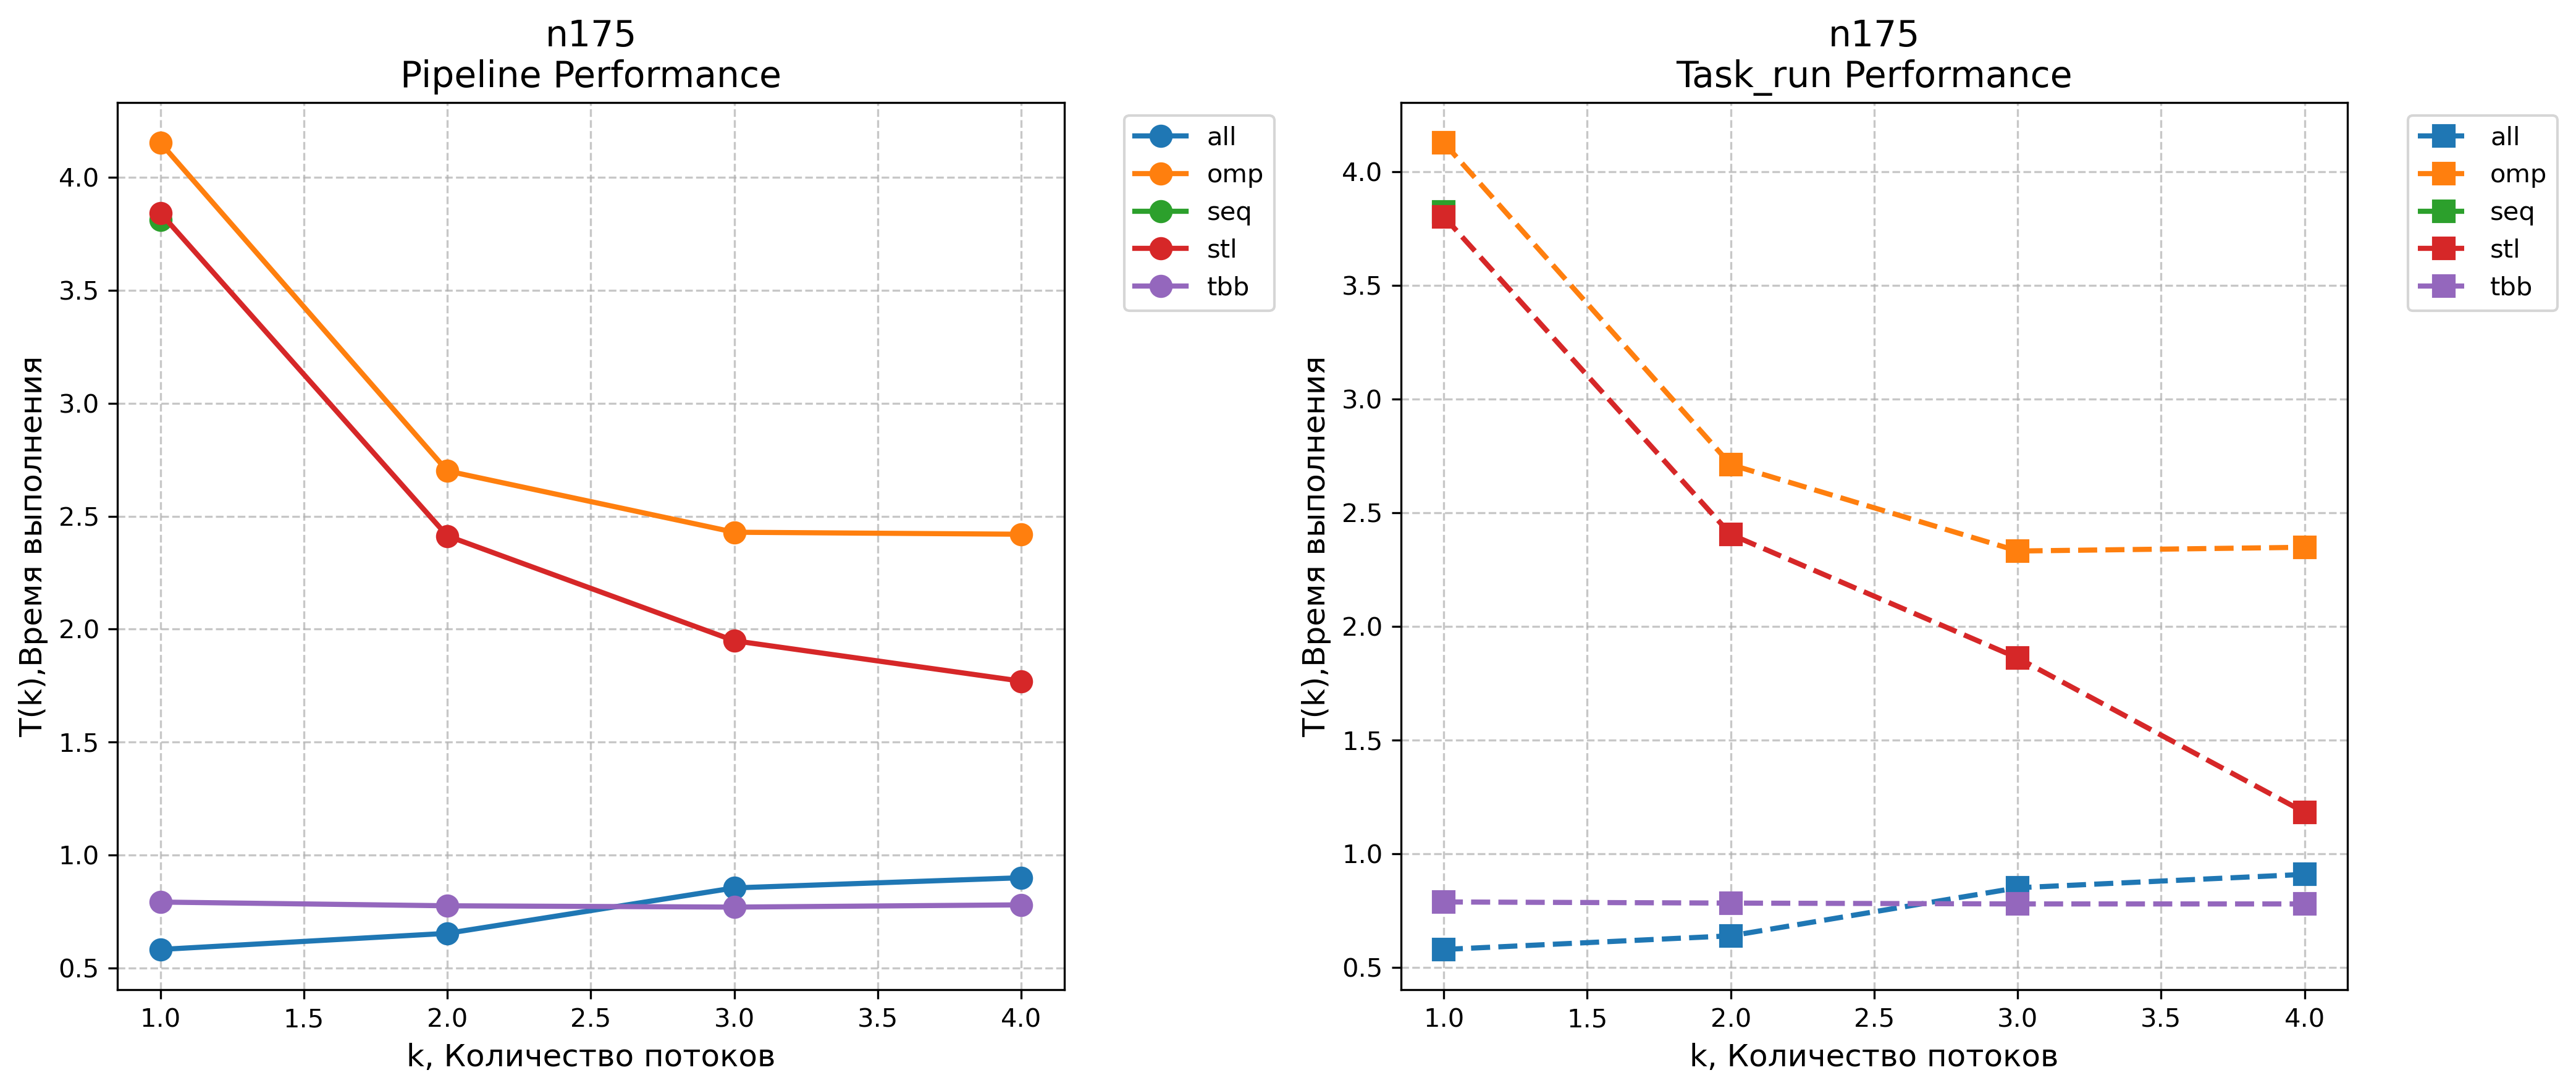
\includegraphics[width=0.8\textwidth]{C:/ppc-2025-threads-reports/tasks/kholin_k_multidim_integrals_rect/ppc_tests/graphics/performance_n175.png}
\caption{Графики производительности для большого объёма данных (n=175)}
\label{fig:large}
\end{figure}


\subsection{Выводы из результатов}
\subsubsection{Сравнение технологий}
С ростом числа потоков у большинства технологий линейно уменьшается время исполнения программы. Это свидетельствует об эффективных параллельных алгоритмах и их можно использовать в дальнейшей разработке. Наибольший прирост производительности наблюдается при переходе от последовательной реализации к параллельной с 2-4 потоками.

\subsubsection{Лучшая производительность}
По результатам экспериментов лучшую производительность показала программа, реализованная с помощью технологии TBB.

\subsubsection{Обоснование лучшей производительности}
Технология TBB демонстрирует стабильную производительность благодаря следующим особенностям:
\begin{itemize}
\item \textbf{Оптимальное распределение нагрузки}: Автоматический планировщик задач (work-stealing scheduler) эффективно балансирует нагрузку между потоками
\item \textbf{Минимизация накладных расходов}
\item \textbf{Кэш-дружественная архитектура}: Алгоритм учитывает локальность данных, минимизируя кэш-промахи
\item \textbf{Гибкий grain size}: Автоматический подбор размера блока итераций (auto\_partitioner)
\end{itemize}
\newpage

\section{ЗАКЛЮЧЕНИЕ}
По итогам работы были реализованы многопоточные программы с применением технологий
OpenMP, TBB, std::thread и MPI + OpenMP, а именно составлено подробное описание каждого алгоритма, обозначены основные принципы работы схем параллельного алгоритма и написан код реализации. Для определения лучшей технологии были проведены эксперименты, подтверждающие эффективность работы перед последовательной версией, а также приведено обоснование лучшей производительности. В настоящем отчёте я считаю все задачи выполненными,а цель - достигнутой. 

\newpage

\section{СПИСОК ЛИТЕРАТУРЫ}

\begin{enumerate}
\item ГОСТ 7.32-2017. Отчет о научно-исследовательской работе. Структура и правила оформления. - М.: Стандартинформ, 2017. - 81 с.

\item Гергель В.П. Теория и практика параллельных вычислений. - М.: Интернет-Университет Информационных Технологий, 2007. - 512 с.

\item Дотч У. Введение в OpenMP. - М.: Издательство МГУ, 2010. - 128 с.

\item Реусенко Д.В. Параллельное программирование с использованием технологии TBB. - СПб.: БХВ-Петербург, 2014. - 288 с.

\item Грушо А.А. Параллельное программирование на основе стандарта MPI. - М.: Издательство МГУ, 2002. - 240 с.

\item Williams A. C++ Concurrency in Action. - Manning Publications, 2019. - 592 p.

\item Chandra R. Parallel Programming in OpenMP. - Morgan Kaufmann, 2001. - 230 p.

\item Voss M. Pro TBB: C++ Parallel Programming with Threading Building Blocks. - Apress, 2019. - 675 p.

\item MPI Forum. MPI: A Message-Passing Interface Standard. Version 4.0, 2021. - 866 p.

\item OpenMP Architecture Review Board. OpenMP Application Programming Interface. Version 5.2, 2021. - 622 p.
\end{enumerate}

\newpage

\section{ПРИЛОЖЕНИЕ}

{\raggedright\textit{\large\bfseries ПРИЛОЖЕНИЕ А}\par}
\addcontentsline{toc}{subsection}{ПРИЛОЖЕНИЕ А}

\textit{Sequential implementation}

\begin{framed}
\begin{lstlisting}[language=C++]

double kholin_k_multidimensional_integrals_rectangle_seq::TestTaskSequential::Integrate(
    const Function& f, const std::vector<double>& l_limits, const std::vector<double>& u_limits,
    const std::vector<double>& h, std::vector<double> f_values, int curr_index_dim, size_t dim, double n) {
  if (curr_index_dim == static_cast<int>(dim)) {
    return f(f_values);
  }

  double sum = 0.0;
  for (int i = 0.0; i < static_cast<int>(n); ++i) {
    f_values[curr_index_dim] = l_limits[curr_index_dim] + (static_cast<double>(i) + 0.5) * h[curr_index_dim];
    sum += Integrate(f, l_limits, u_limits, h, f_values, curr_index_dim + 1, dim, n);
  }
  return sum * h[curr_index_dim];
}

double kholin_k_multidimensional_integrals_rectangle_seq::TestTaskSequential::IntegrateWithRectangleMethod(
    const Function& f, std::vector<double>& f_values, const std::vector<double>& l_limits,
    const std::vector<double>& u_limits, size_t dim, double n, std::vector<double> h) {
  for (size_t i = 0; i < dim; ++i) {
    h[i] = (u_limits[i] - l_limits[i]) / n;
  }

  return Integrate(f, l_limits, u_limits, h, f_values, 0, dim, n);
}

double kholin_k_multidimensional_integrals_rectangle_seq::TestTaskSequential::RunMultistepSchemeMethodRectangle(
    const Function& f, std::vector<double> f_values, const std::vector<double>& l_limits,
    const std::vector<double>& u_limits, size_t dim, double n) {
  std::vector<double> h(dim);
  double i_n = 0.0;
  i_n = IntegrateWithRectangleMethod(f, f_values, l_limits, u_limits, dim, n, h);
  return i_n;
}

bool kholin_k_multidimensional_integrals_rectangle_seq::TestTaskSequential::PreProcessingImpl() {
  // Init value for input and output
  sz_values_ = task_data->inputs_count[0];
  sz_lower_limits_ = task_data->inputs_count[1];
  sz_upper_limits_ = task_data->inputs_count[2];

  auto* ptr_dim = reinterpret_cast<size_t*>(task_data->inputs[0]);
  dim_ = *ptr_dim;

  auto* ptr_f_values = reinterpret_cast<double*>(task_data->inputs[1]);
  f_values_.assign(ptr_f_values, ptr_f_values + sz_values_);

  auto* ptr_f = reinterpret_cast<std::function<double(const std::vector<double>&)>*>(task_data->inputs[2]);
  f_ = *ptr_f;

  auto* ptr_lower_limits = reinterpret_cast<double*>(task_data->inputs[3]);
  lower_limits_.assign(ptr_lower_limits, ptr_lower_limits + sz_lower_limits_);

  auto* ptr_upper_limits = reinterpret_cast<double*>(task_data->inputs[4]);
  upper_limits_.assign(ptr_upper_limits, ptr_upper_limits + sz_upper_limits_);

  auto* ptr_start_n = reinterpret_cast<double*>(task_data->inputs[5]);
  start_n_ = *ptr_start_n;

  result_ = 0.0;
  return true;
}

bool kholin_k_multidimensional_integrals_rectangle_seq::TestTaskSequential::ValidationImpl() {
  // Check equality of counts elements
  return task_data->inputs_count[1] > 0U && task_data->inputs_count[2] > 0U;
}

bool kholin_k_multidimensional_integrals_rectangle_seq::TestTaskSequential::RunImpl() {
  result_ = RunMultistepSchemeMethodRectangle(f_, f_values_, lower_limits_, upper_limits_, dim_, start_n_);
  return true;
}

bool kholin_k_multidimensional_integrals_rectangle_seq::TestTaskSequential::PostProcessingImpl() {
  reinterpret_cast<double*>(task_data->outputs[0])[0] = result_;
  return true;
}

\end{lstlisting}
\end{framed}


\newpage

{\raggedright\textit{\large\bfseries ПРИЛОЖЕНИЕ Б}\par}
\addcontentsline{toc}{subsection}{ПРИЛОЖЕНИЕ Б}

\textit{OpenMP implementation}

\begin{framed}
\begin{lstlisting}[language=C++]

double kholin_k_multidimensional_integrals_rectangle_omp::TestTaskOpenMP::Integrate(
    const Function& f, const std::vector<double>& l_limits, const std::vector<double>& u_limits,
    const std::vector<double>& h, std::vector<double> f_values, int curr_index_dim, size_t dim, double n) {
  if (curr_index_dim == static_cast<int>(dim)) {
    return f(f_values);
  }

  double sum = 0.0;
#pragma omp parallel for reduction(+ : sum) schedule(dynamic)
  for (int i = 0.0; i < static_cast<int>(n); ++i) {
    f_values[curr_index_dim] = l_limits[curr_index_dim] + (static_cast<double>(i) + 0.5) * h[curr_index_dim];
    sum += Integrate(f, l_limits, u_limits, h, f_values, curr_index_dim + 1, dim, n);
  }
  return sum * h[curr_index_dim];
}

double kholin_k_multidimensional_integrals_rectangle_omp::TestTaskOpenMP::IntegrateWithRectangleMethod(
    const Function& f, std::vector<double>& f_values, const std::vector<double>& l_limits,
    const std::vector<double>& u_limits, size_t dim, double n, std::vector<double> h) {
  for (size_t i = 0; i < dim; ++i) {
    h[i] = (u_limits[i] - l_limits[i]) / n;
  }

  return Integrate(f, l_limits, u_limits, h, f_values, 0, dim, n);
}

double kholin_k_multidimensional_integrals_rectangle_omp::TestTaskOpenMP::RunMultistepSchemeMethodRectangle(
    const Function& f, std::vector<double> f_values, const std::vector<double>& l_limits,
    const std::vector<double>& u_limits, size_t dim, double n) {
  std::vector<double> h(dim);
  double i_n = 0.0;
  i_n = IntegrateWithRectangleMethod(f, f_values, l_limits, u_limits, dim, n, h);
  return i_n;
}

bool kholin_k_multidimensional_integrals_rectangle_omp::TestTaskOpenMP::PreProcessingImpl() {
  // Init value for input and output
  sz_values_ = task_data->inputs_count[0];
  sz_lower_limits_ = task_data->inputs_count[1];
  sz_upper_limits_ = task_data->inputs_count[2];

  auto* ptr_dim = reinterpret_cast<size_t*>(task_data->inputs[0]);
  dim_ = *ptr_dim;

  auto* ptr_f_values = reinterpret_cast<double*>(task_data->inputs[1]);
  f_values_.assign(ptr_f_values, ptr_f_values + sz_values_);

  auto* ptr_f = reinterpret_cast<std::function<double(const std::vector<double>&)>*>(task_data->inputs[2]);
  f_ = *ptr_f;

  auto* ptr_lower_limits = reinterpret_cast<double*>(task_data->inputs[3]);
  lower_limits_.assign(ptr_lower_limits, ptr_lower_limits + sz_lower_limits_);

  auto* ptr_upper_limits = reinterpret_cast<double*>(task_data->inputs[4]);
  upper_limits_.assign(ptr_upper_limits, ptr_upper_limits + sz_upper_limits_);

  auto* ptr_start_n = reinterpret_cast<double*>(task_data->inputs[5]);
  start_n_ = *ptr_start_n;

  result_ = 0.0;
  return true;
}

bool kholin_k_multidimensional_integrals_rectangle_omp::TestTaskOpenMP::ValidationImpl() {
  // Check equality of counts elements
  return task_data->inputs_count[1] > 0U && task_data->inputs_count[2] > 0U;
}

bool kholin_k_multidimensional_integrals_rectangle_omp::TestTaskOpenMP::RunImpl() {
  result_ = RunMultistepSchemeMethodRectangle(f_, f_values_, lower_limits_, upper_limits_, dim_, start_n_);
  return true;
}

bool kholin_k_multidimensional_integrals_rectangle_omp::TestTaskOpenMP::PostProcessingImpl() {
  reinterpret_cast<double*>(task_data->outputs[0])[0] = result_;
  return true;
}

\end{lstlisting}
\end{framed}

\newpage

{\raggedright\textit{\large\bfseries ПРИЛОЖЕНИЕ В}\par}
\addcontentsline{toc}{subsection}{ПРИЛОЖЕНИЕ В}

\textit{TBB implementation}

\begin{framed}
\begin{lstlisting}[language=C++]

double kholin_k_multidimensional_integrals_rectangle_tbb::TestTaskTBB::Integrate(
    const Function& f, const std::vector<double>& l_limits, const std::vector<double>& u_limits,
    const std::vector<double>& h, std::vector<double>& f_values, int curr_index_dim, size_t dim, double n) {
  if (curr_index_dim == static_cast<int>(dim)) {
    return f(f_values);
  }

  const double step = h[curr_index_dim];
  const double start_pos = l_limits[curr_index_dim] + (0.5 * step);

  return tbb::parallel_reduce(
             tbb::blocked_range<int>(0, static_cast<int>(n), 1000), 0.0,
             [&](const tbb::blocked_range<int>& r, double local_sum) {
               std::vector<double> local_f_values = f_values;
               for (int i = r.begin(); i < r.end(); ++i) {
                 local_f_values[curr_index_dim] = start_pos + static_cast<double>(i) * step;
                 local_sum += Integrate(f, l_limits, u_limits, h, local_f_values, curr_index_dim + 1, dim, n);
               }
               return local_sum;
             },
             std::plus<>(), tbb::auto_partitioner()) *
         step;
}

double kholin_k_multidimensional_integrals_rectangle_tbb::TestTaskTBB::IntegrateWithRectangleMethod(
    const Function& f, std::vector<double>& f_values, const std::vector<double>& l_limits,
    const std::vector<double>& u_limits, size_t dim, double n, std::vector<double>& h) {
  for (size_t i = 0; i < dim; ++i) {
    h[i] = (u_limits[i] - l_limits[i]) / n;
  }
  return kholin_k_multidimensional_integrals_rectangle_tbb::TestTaskTBB::Integrate
  (f, l_limits, u_limits, h, f_values, 0, dim, n);
}

double kholin_k_multidimensional_integrals_rectangle_tbb::TestTaskTBB::RunMultistepSchemeMethodRectangle(
    const Function& f, std::vector<double> f_values, const std::vector<double>& l_limits,
    const std::vector<double>& u_limits, size_t dim, double n) {
  std::vector<double> h(dim);
  return kholin_k_multidimensional_integrals_rectangle_tbb::TestTaskTBB::IntegrateWithRectangleMethod(
      f, f_values, l_limits, u_limits, dim, n, h);
}

bool kholin_k_multidimensional_integrals_rectangle_tbb::TestTaskTBB::PreProcessingImpl() {
  sz_values_ = task_data->inputs_count[0];
  sz_lower_limits_ = task_data->inputs_count[1];
  sz_upper_limits_ = task_data->inputs_count[2];

  auto* ptr_dim = reinterpret_cast<size_t*>(task_data->inputs[0]);
  dim_ = *ptr_dim;

  auto* ptr_f_values = reinterpret_cast<double*>(task_data->inputs[1]);
  f_values_.assign(ptr_f_values, ptr_f_values + sz_values_);

  auto* ptr_f = reinterpret_cast<std::function<double(const std::vector<double>&)>*>(task_data->inputs[2]);
  f_ = *ptr_f;

  auto* ptr_lower_limits = reinterpret_cast<double*>(task_data->inputs[3]);
  lower_limits_.assign(ptr_lower_limits, ptr_lower_limits + sz_lower_limits_);

  auto* ptr_upper_limits = reinterpret_cast<double*>(task_data->inputs[4]);
  upper_limits_.assign(ptr_upper_limits, ptr_upper_limits + sz_upper_limits_);

  auto* ptr_start_n = reinterpret_cast<double*>(task_data->inputs[5]);
  start_n_ = *ptr_start_n;

  result_ = 0.0;
  return true;
}

bool kholin_k_multidimensional_integrals_rectangle_tbb::TestTaskTBB::ValidationImpl() {
  return task_data->inputs_count[1] > 0U && task_data->inputs_count[2] > 0U;
}

bool kholin_k_multidimensional_integrals_rectangle_tbb::TestTaskTBB::RunImpl() {
  result_ = kholin_k_multidimensional_integrals_rectangle_tbb::TestTaskTBB::
                RunMultistepSchemeMethodRectangle(
      f_, f_values_, lower_limits_, upper_limits_, dim_, start_n_);
  return true;
}

bool kholin_k_multidimensional_integrals_rectangle_tbb::TestTaskTBB::PostProcessingImpl() {
  reinterpret_cast<double*>(task_data->outputs[0])[0] = result_;
  return true;
}

\end{lstlisting}
\end{framed}

\newpage

{\raggedright\textit{\large\bfseries ПРИЛОЖЕНИЕ Г}\par}
\addcontentsline{toc}{subsection}{ПРИЛОЖЕНИЕ Г}

\textit{std::thread implementation}

\begin{framed}
\begin{lstlisting}[language=C++]

double kholin_k_multidimensional_integrals_rectangle_stl::TestTaskSTL::Integrate(
    const Function& f, const std::vector<double>& l_limits, const std::vector<double>& u_limits,
    const std::vector<double>& h, std::vector<double> f_values, int curr_index_dim, size_t dim, double n) {
  if (curr_index_dim == static_cast<int>(dim)) {
    return f(f_values);
  }

  const int total_steps = static_cast<int>(n);
  double sum = 0.0;

  if (curr_index_dim == 0) {
    const int num_threads = ppc::util::GetPPCNumThreads();
    std::vector<std::thread> threads(num_threads);
    std::vector<double> thread_sums(num_threads, 0.0);

    const int base_steps = total_steps / num_threads;
    const int remainder = total_steps % num_threads;

    for (int t = 0; t < num_threads; ++t) {
      const int start = (t * base_steps) + (t < remainder ? t : remainder);
      const int end = start + base_steps + (t < remainder ? 1 : 0);

      threads[t] = std::thread([&, start, end, t]() {
        std::vector<double> local_f_values = f_values;
        double local_sum = 0.0;
        for (int i = start; i < end; ++i) {
          local_f_values[0] = l_limits[0] + (i + 0.5) * h[0];
          local_sum += Integrate(f, l_limits, u_limits, h, local_f_values, 1, dim, n);
        }
        thread_sums[t] = local_sum;
      });
    }

    for (auto& th : threads) {
      if (th.joinable()) {
        th.join();
      }
    }
    sum = std::accumulate(thread_sums.begin(), thread_sums.end(), 0.0) * h[0];
  } else {
    for (int i = 0; i < total_steps; ++i) {
      f_values[curr_index_dim] = l_limits[curr_index_dim] + (i + 0.5) * h[curr_index_dim];
      sum += Integrate(f, l_limits, u_limits, h, f_values, curr_index_dim + 1, dim, n);
    }
    sum *= h[curr_index_dim];
  }

  return sum;
}

double kholin_k_multidimensional_integrals_rectangle_stl::TestTaskSTL::IntegrateWithRectangleMethod(
    const Function& f, std::vector<double>& f_values, const std::vector<double>& l_limits,
    const std::vector<double>& u_limits, size_t dim, double n, std::vector<double> h) {
  for (size_t i = 0; i < dim; ++i) {
    h[i] = (u_limits[i] - l_limits[i]) / n;
  }

  return Integrate(f, l_limits, u_limits, h, f_values, 0, dim, n);
}

double kholin_k_multidimensional_integrals_rectangle_stl::TestTaskSTL::RunMultistepSchemeMethodRectangle(
    const Function& f, std::vector<double> f_values, const std::vector<double>& l_limits,
    const std::vector<double>& u_limits, size_t dim, double n) {
  std::vector<double> h(dim);
  double i_n = 0.0;

  i_n = IntegrateWithRectangleMethod(f, f_values, l_limits, u_limits, dim, n, h);
  return i_n;
}

bool kholin_k_multidimensional_integrals_rectangle_stl::TestTaskSTL::PreProcessingImpl() {
  // Init value for input and output
  sz_values_ = task_data->inputs_count[0];
  sz_lower_limits_ = task_data->inputs_count[1];
  sz_upper_limits_ = task_data->inputs_count[2];

  auto* ptr_dim = reinterpret_cast<size_t*>(task_data->inputs[0]);
  dim_ = *ptr_dim;

  auto* ptr_f_values = reinterpret_cast<double*>(task_data->inputs[1]);
  f_values_.assign(ptr_f_values, ptr_f_values + sz_values_);

  auto* ptr_f = reinterpret_cast<std::function<double(const std::vector<double>&)>*>(task_data->inputs[2]);
  f_ = *ptr_f;

  auto* ptr_lower_limits = reinterpret_cast<double*>(task_data->inputs[3]);
  lower_limits_.assign(ptr_lower_limits, ptr_lower_limits + sz_lower_limits_);

  auto* ptr_upper_limits = reinterpret_cast<double*>(task_data->inputs[4]);
  upper_limits_.assign(ptr_upper_limits, ptr_upper_limits + sz_upper_limits_);

  auto* ptr_start_n = reinterpret_cast<double*>(task_data->inputs[5]);
  start_n_ = *ptr_start_n;

  result_ = 0.0;
  count_level_par_ = 1;
  return true;
}

bool kholin_k_multidimensional_integrals_rectangle_stl::TestTaskSTL::ValidationImpl() {
  // Check equality of counts elements
  return task_data->inputs_count[1] > 0U && task_data->inputs_count[2] > 0U;
}

bool kholin_k_multidimensional_integrals_rectangle_stl::TestTaskSTL::RunImpl() {
  result_ = RunMultistepSchemeMethodRectangle(f_, f_values_, lower_limits_, upper_limits_, dim_, start_n_);
  return true;
}

bool kholin_k_multidimensional_integrals_rectangle_stl::TestTaskSTL::PostProcessingImpl() {
  reinterpret_cast<double*>(task_data->outputs[0])[0] = result_;
  return true;
}

\end{lstlisting}
\end{framed}

\newpage

{\raggedright\textit{\large\bfseries ПРИЛОЖЕНИЕ Г}\par}
\addcontentsline{toc}{subsection}{ПРИЛОЖЕНИЕ Г}

\textit{MPI + OMP implementation}

\begin{framed}
\begin{lstlisting}[language=C++]

double kholin_k_multidimensional_integrals_rectangle_all::TestTaskALL::Integrate(
    const Function& f, const std::vector<double>& l_limits, const std::vector<double>& u_limits,
    const std::vector<double>& h, std::vector<double>& f_values, int curr_index_dim, int dim, double n) {
  if (curr_index_dim == dim) {
    return f(f_values);
  }

  double sum = 0.0;
  const double l_limit = l_limits[curr_index_dim];
  const double step = h[curr_index_dim];

  for (int i = 0; i < static_cast<int>(n); ++i) {
    f_values[curr_index_dim] = l_limit + (static_cast<double>(i) + 0.5) * step;
    sum += Integrate(f, l_limits, u_limits, h, f_values, curr_index_dim + 1, dim, n);
  }
  return sum * h[curr_index_dim];
}

double kholin_k_multidimensional_integrals_rectangle_all::TestTaskALL::IntegrateWithRectangleMethod(
    const Function& f, std::vector<double>& f_values, const std::vector<double>& l_limits,
    const std::vector<double>& u_limits, int dim, double n) {
  std::vector<double> h(dim);
#pragma omp parallel for
  for (int i = 0; i < dim; ++i) {
    h[i] = (u_limits[i] - l_limits[i]) / n;
  }
  return Integrate(f, l_limits, u_limits, h, f_values, 0, dim, n);
}

double kholin_k_multidimensional_integrals_rectangle_all::TestTaskALL::RunMultistepSchemeMethodRectangle(
    const Function& f, std::vector<double>& f_values, const std::vector<double>& l_limits,
    const std::vector<double>& u_limits, int dim, double n) {
  int rank = 0;
  int size = 0;
  MPI_Comm_size(MPI_COMM_WORLD, &size);
  MPI_Comm_rank(MPI_COMM_WORLD, &rank);
  if (rank >= 0) {
    local_l_limits_ = std::vector<double>(dim);
    local_u_limits_ = std::vector<double>(dim);
  }
  for (int i = 0; i < dim_; ++i) {
    double range = u_limits[i] - l_limits[i];
    local_l_limits_[i] = l_limits[i] + (rank * (range / size));
    local_u_limits_[i] = l_limits[i] + ((rank + 1) * (range / size));
  }
  double local_result = IntegrateWithRectangleMethod(f, f_values, local_l_limits_, local_u_limits_, dim, n);
  if (dim_ > 1) {
    local_result = local_result * std::pow(size, dim - 1);
  }
  MPI_Reduce(&local_result, &I_2n_, 1, MPI_DOUBLE, MPI_SUM, 0, MPI_COMM_WORLD);
  return I_2n_;
}

bool kholin_k_multidimensional_integrals_rectangle_all::TestTaskALL::PreProcessingImpl() {
  int rank = 0;
  int size = 0;
  MPI_Comm_size(MPI_COMM_WORLD, &size);
  MPI_Comm_rank(MPI_COMM_WORLD, &rank);
  if (rank == 0) {
    // Init value for input and output
    sz_values_ = static_cast<int>(task_data->inputs_count[0]);
    sz_lower_limits_ = static_cast<int>(task_data->inputs_count[1]);
    sz_upper_limits_ = static_cast<int>(task_data->inputs_count[2]);

    auto* ptr_dim = reinterpret_cast<int*>(task_data->inputs[0]);
    dim_ = *ptr_dim;

    auto* ptr_f_values = reinterpret_cast<double*>(task_data->inputs[1]);
    f_values_.assign(ptr_f_values, ptr_f_values + sz_values_);

    auto* ptr_lower_limits = reinterpret_cast<double*>(task_data->inputs[2]);
    lower_limits_.assign(ptr_lower_limits, ptr_lower_limits + sz_lower_limits_);

    auto* ptr_upper_limits = reinterpret_cast<double*>(task_data->inputs[3]);
    upper_limits_.assign(ptr_upper_limits, ptr_upper_limits + sz_upper_limits_);

    auto* ptr_start_n = reinterpret_cast<double*>(task_data->inputs[4]);
    start_n_ = *ptr_start_n;
  }
  return true;
}

bool kholin_k_multidimensional_integrals_rectangle_all::TestTaskALL::ValidationImpl() {
  int rank = 0;
  MPI_Comm_rank(MPI_COMM_WORLD, &rank);
  if (rank == 0) {
    return task_data->inputs_count[1] > 0U && task_data->inputs_count[2] > 0U;
  }
  return true;
}

bool kholin_k_multidimensional_integrals_rectangle_all::TestTaskALL::RunImpl() {
  int size = 0;
  int rank = 0;
  MPI_Comm_size(MPI_COMM_WORLD, &size);
  MPI_Comm_rank(MPI_COMM_WORLD, &rank);

  MPI_Bcast(&sz_values_, 1, MPI_INT, 0, MPI_COMM_WORLD);
  MPI_Bcast(&sz_lower_limits_, 1, MPI_INT, 0, MPI_COMM_WORLD);
  MPI_Bcast(&sz_upper_limits_, 1, MPI_INT, 0, MPI_COMM_WORLD);
  MPI_Bcast(&dim_, 1, MPI_INT, 0, MPI_COMM_WORLD);
  MPI_Bcast(&start_n_, 1, MPI_DOUBLE, 0, MPI_COMM_WORLD);

  if (rank > 0) {
    f_values_ = std::vector<double>(sz_values_);
    lower_limits_ = std::vector<double>(sz_lower_limits_);
    upper_limits_ = std::vector<double>(sz_upper_limits_);
  }
  MPI_Bcast(lower_limits_.data(), sz_lower_limits_, MPI_DOUBLE, 0, MPI_COMM_WORLD);
  MPI_Bcast(upper_limits_.data(), sz_upper_limits_, MPI_DOUBLE, 0, MPI_COMM_WORLD);
  MPI_Bcast(f_values_.data(), sz_values_, MPI_DOUBLE, 0, MPI_COMM_WORLD);

  RunMultistepSchemeMethodRectangle(f_, f_values_, lower_limits_, upper_limits_, dim_, start_n_);
  return true;
}

bool kholin_k_multidimensional_integrals_rectangle_all::TestTaskALL::PostProcessingImpl() {
  int rank = 0;
  MPI_Comm_rank(MPI_COMM_WORLD, &rank);
  if (rank == 0) {
    reinterpret_cast<double*>(task_data->outputs[0])[0] = I_2n_;
  }
  return true;
}


\end{lstlisting}
\end{framed}

\end{document}